\section*{Demostración de Optimalidad: Algoritmo Greedy}

Para demostrar que nuestra estrategia Greedy (ordenar los videos de forma descendente según el tiempo del ayudante $a_i$) es óptima, utilizaremos método de inversiones.

\subsection*{Definiciones}
Sea $S$ un conjunto de $n$ rivales a analizar. Para cada rival $i$, definimos:
\begin{itemize}
    \item $s_i$: Tiempo que le toma a Scaloni analizar el rival $i$.
    \item $a_i$: Tiempo que le toma al ayudante analizar el rival $i$.
\end{itemize}
El tiempo de finalización de un rival $i$ depende de la suma de los tiempos de Scaloni de todos los rivales anteriores, más $s_i$ y $a_i$. El objetivo es minimizar el tiempo máximo en el que terminan los ayudantes y Scaloni.

\subsection*{Hipótesis}
Nuestra solución Greedy se basa en ordenar de forma descendente a los pares ($s_i$, $a_i$), de forma tal que los primeros rivales a ser analizados son los que tienen mayor tiempo de análisis por ayudante. Es importante recalcar que el análisis de los rivales se produce sin tiempo de desuso. Se espera que con esta estrategia de ordenamiento, el tiempo máximo en el que Scaloni y sus ayudantes pueden analizar a todos sus rivales sea el mínimo. 

Por lo tanto, para cada par de rivales en nuestra solución propuesta es:

$$a_i > a_j > ... > a_n$$


Vamos a probar que la solución Greedy da siempre un orden óptimo utilizando el método de inversiones.


\subsection*{Definición de Inversión}
Supongamos que existe un algoritmo $O$ óptimo distinto a la solución Greedy propuesta. Si $O$ tiene una inversión, entonces existe un par de rivales a procesar $i$ y $j$ en el que $j$ fue analizado inmediatamente después de $i$ (primero $i$, luego $j$) de tal forma que presentan una inversión respecto a la regla Greedy:
$$a_i < a_j$$
Supongamos que Scaloni comienza a analizar el rival $i$ en un tiempo acumulado $T$. 

\newpage

\subsection*{Análisis del Cronograma Óptimo $O$}
Los tiempos de finalización para este par de tareas en $O$ son:
\begin{itemize}
    \item El ayudante termina el rival $i$ en: $C_i = T + s_i + a_i$
    \item El ayudante termina el rival $j$ en: $C_j = T + s_i + s_j + a_j$
\end{itemize}
El tiempo máximo para este bloque en $O$ es el máximo entre $C_i$ y $C_j$. Como $s_j > 0$ y por nuestra hipótesis de inversión $a_j > a_i$, es evidente que:
$$\text{Max}_{O} = \max(T + s_i + a_i, \, T + s_i + s_j + a_j) = T + s_i + s_j + a_j$$

\subsection*{El Intercambio (Cronograma $O'$)}
Construimos un nuevo cronograma $O'$ intercambiando únicamente el orden de $i$ y $j$ (primero $j$, luego $i$), dejando el resto intacto. Los nuevos tiempos de finalización son:
\begin{itemize}
    \item El ayudante termina el rival $j$ en: $C'_j = T + s_j + a_j$
    \item El ayudante termina el rival $i$ en: $C'_i = T + s_j + s_i + a_i$
\end{itemize}
El tiempo máximo para este bloque en el nuevo cronograma $O'$ es:
$$\text{Max}_{O'} = \max(T + s_j + a_j, \, T + s_j + s_i + a_i)$$

\subsection*{Comparación de optimalidad}
Comparamos ambos términos de $\text{Max}_{O'}$ con $\text{Max}_{O}$:
\begin{enumerate}
    \item $T + s_j + a_j < T + s_i + s_j + a_j$ (ya que $s_i > 0$).
    \item $T + s_j + s_i + a_i < T + s_i + s_j + a_j$ (ya que $a_i < a_j$ por la inversión).
\end{enumerate}

Ambos tiempos posibles de finalización en $O'$ son estrictamente menores al tiempo de finalización en $O$. Además, como ambos rivales en conjunto siguen consumiendo exactamente $s_i + s_j$ del tiempo de Scaloni, el tiempo de inicio de todos los rivales posteriores no se ve afectado.

Por lo tanto, el \textit{tiempo máximo} de $O'$ es menor o igual al de $O$. Como $O$ era óptimo, $O'$ también debe serlo. Repitiendo este proceso para deshacer cada inversión, llegaremos exactamente a nuestro ordenamiento Greedy sin aumentar el tiempo total. 

Esto explica matemáticamente por qué el tiempo global de nuestro nuevo cronograma $O'$ será \textbf{menor o igual} ($\le$) al de $O$. Pueden existir configuraciones óptimas con inversiones inofensivas que no penalizan el tiempo global, pero el intercambio demuestra rigurosamente que llevar cualquier configuración a su forma Greedy jamás empeorará el resultado. $\blacksquare$

\newpage

\subsection*{Análisis de Múltiples Óptimos y Tiempo Global}
Es fundamental notar la diferencia entre el tiempo máximo \textit{local} del bloque intercambiado y el tiempo de finalización \textit{global} de todo el proyecto. 

Supongamos un escenario genérico donde existe una tarea inicial tan demandante para un ayudante que define, por sí sola, el tiempo de finalización de todo el proyecto (un gran cuello de botella). Si más adelante en el cronograma existe un par de tareas invertidas (una corta seguida de una más larga), deshacer esa inversión mejorará estrictamente el tiempo \textit{local} de ese par. Sin embargo, como el tiempo de ese pequeño bloque queda ``oculto'' o absorbido por la larga espera de la tarea gigante inicial, el tiempo \textit{global} del proyecto se mantendrá exactamente igual.

\begin{figure}[H]
    \centering
    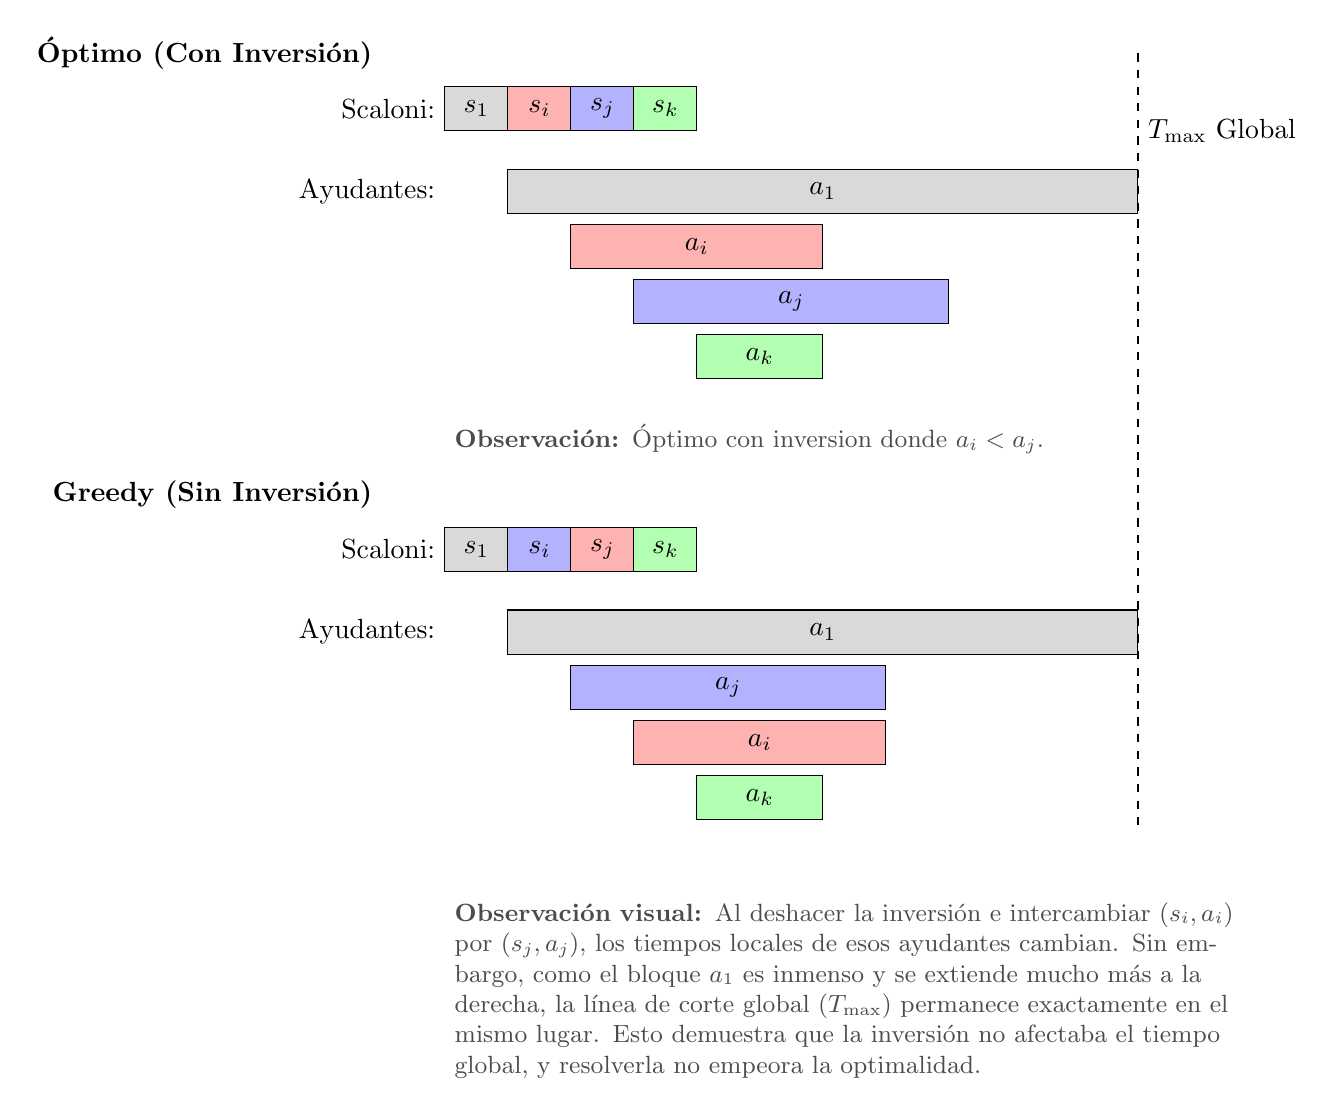
\begin{tikzpicture}[x=0.8cm, y=0.7cm]
        
        % ==========================================
        % CRONOGRAMA 1: Óptimo (Con Inversión)
        % ==========================================
        \node[anchor=east, font=\bfseries] at (-1, 0) {Óptimo (Con Inversión)};
        
        % Eje Scaloni
        \node[anchor=east] at (0, -1) {Scaloni:};
        \draw[fill=gray!30] (0,-1.4) rectangle (1,-0.6) node[midway] {$s_1$};
        \draw[fill=red!30]  (1,-1.4) rectangle (2,-0.6) node[midway] {$s_i$};
        \draw[fill=blue!30] (2,-1.4) rectangle (3,-0.6) node[midway] {$s_j$};
        \draw[fill=green!30](3,-1.4) rectangle (4,-0.6) node[midway] {$s_k$};
        
        % Ejes Ayudantes
        \node[anchor=east] at (0, -2.5) {Ayudantes:};
        % Ayudante 1
        \draw[fill=gray!30] (1,-2.9) rectangle (11,-2.1) node[midway] {$a_1$};
        % Ayudante x
        \draw[fill=red!30]  (2,-3.9) rectangle (6,-3.1) node[midway] {$a_i$};
        % Ayudante y
        \draw[fill=blue!30] (3,-4.9) rectangle (8,-4.1) node[midway] {$a_j$};
        % Ayudante z
        \draw[fill=green!30](4,-5.9) rectangle (6,-5.1) node[midway] {$a_k$};

        % Línea de Tiempo Máximo
        \draw[dashed, thick] (11, 0) -- (11, -14) node[pos=0.1, right] {$T_{\max}$ Global};

        \node[anchor=west, text width=10cm, font=\small, text=black!70] at (0, -7) {
            \textbf{Observación:} Óptimo con inversion donde $a_i < a_j$.
        };

        % ==========================================
        % CRONOGRAMA 2: Greedy (Sin Inversión)
        % ==========================================
        \node[anchor=east, font=\bfseries] at (-1, -8) {Greedy (Sin Inversión)};
        
        % Eje Scaloni
        \node[anchor=east] at (0, -9) {Scaloni:};
        \draw[fill=gray!30] (0,-9.4) rectangle (1,-8.6) node[midway] {$s_1$};
        \draw[fill=blue!30] (1,-9.4) rectangle (2,-8.6) node[midway] {$s_i$};
        \draw[fill=red!30]  (2,-9.4) rectangle (3,-8.6) node[midway] {$s_j$};
        \draw[fill=green!30](3,-9.4) rectangle (4,-8.6) node[midway] {$s_k$};
        
        % Ejes Ayudantes
        \node[anchor=east] at (0, -10.5) {Ayudantes:};
        % Ayudante 1
        \draw[fill=gray!30] (1,-10.9) rectangle (11,-10.1) node[midway] {$a_1$};
        % Ayudante y
        \draw[fill=blue!30] (2,-11.9) rectangle (7,-11.1) node[midway] {$a_j$};
        % Ayudante x
        \draw[fill=red!30]  (3,-12.9) rectangle (7,-12.1) node[midway] {$a_i$};
        % Ayudante z
        \draw[fill=green!30](4,-13.9) rectangle (6,-13.1) node[midway] {$a_k$};
        
        % Notas
        \node[anchor=west, text width=10cm, font=\small, text=black!70] at (0, -17) {
            \textbf{Observación visual:} Al deshacer la inversión e intercambiar $(s_i, a_i)$ por $(s_j, a_j)$, los tiempos locales de esos ayudantes cambian. Sin embargo, como el bloque $a_1$ es inmenso y se extiende mucho más a la derecha, la línea de corte global ($T_{\max}$) permanece exactamente en el mismo lugar. Esto demuestra que la inversión no afectaba el tiempo global, y resolverla no empeora la optimalidad.
        };

    \end{tikzpicture}
    \caption{Comparación visual de los cronogramas con y sin inversión. La tarea $(s_1, a_1)$ enmascara los tiempos locales de $(s_i, a_i)$ y $(s_j, a_j)$.}
    \label{fig:inversiones}
\end{figure}


\subsection*{Conclusión}
Como $O$ era óptimo y demostramos que el tiempo global de $O'$ es menor o igual, $O'$ también debe ser óptimo. Repitiendo este proceso de intercambio para deshacer cada inversión, llegaremos exactamente a nuestro ordenamiento Greedy sin aumentar el tiempo total en ningún paso. Se concluye que el algoritmo Greedy propuesto siempre pertenece al conjunto de soluciones óptimas, minimizando el tiempo global. $\blacksquare$
